\chapter{Introdução}
\label{chap:intro}

Segundo \citeonline{mamede2005}, as linhas de transmissão são elementos de um sistema elétrico que transportam a energia produzida pelas fontes de geração até as subestações abaixadoras instaladas próximas aos grandes centros de carga. Como as fontes de geração
de energia são construídas longes dos centros consumidores é preciso de linhas de transmissão de grandes extensões, o que as tornam susceptíveis às incidências de defeitos.

Um dos maiores problemas na distribuição de energia é o aquecimento anormal associado à alta resistência ou fluxo de corrente excessiva, onde alguns dos componentes afetados são os transformadores trifásicos, switches, conetores, fusíveis, cabos, etc \cite{canahuire}. Outro problema comum é a proximidade de objetos não desejados dos cabos de alta tensão, que podem acarretar em curtos circuitos fase-terra no sistema elétrico de potência

No Brasil, existe uma quantidade considerável de linhas de transmissão de alta tensão que já ultrapassaram a vida útil das quais foram destinadas. Com a degradação dos componentes nela instalados, que podem causar possíveis problemas, vê-se a necessidade de manutenções preditivas a fim de verificar a integridade do sistema.

Atualmente, a inspeção de linhas de transmissão é feita através de aeronaves tripuladas e uma equipe especializada. Essas inspeções são relativamente custosas e não possuem uma boa eficiência, por ser uma inspeção visual. Há também um risco associado a esta tarefa, pois as aeronaves precisam sobrevoar próximos a LT para que um operador para realize o procedimento, como pode ser vista na figura \ref{lineinspection}.

Umas das técnicas comumente utilizada para inspeção de linhas de transmissão é a termografia, capaz de identificar o aumento de temperatura nos cabos e equipamentos.  A inspeção por câmera térmica é de suma importância para a integridade dos equipamentos, já que por sua vez podem identificar possíveis problemas. Vale ressaltar que as inspeções não verificam apenas os equipamentos, mas monitoram se há algum impedimento na faixa de servidão, visto que construções e vegetação necessitam manter uma distância mínima da mesma. Uma exemplo de faixa de servidão pode ser observada na Figura \ref{linhaservidao}.
%sugiro que vc acrescente observações quanto as outras inspeções, parece que vc irá fazer a inspeção da área de servidão com a IR cam

\begin{figure}[!ht]
	\centering
	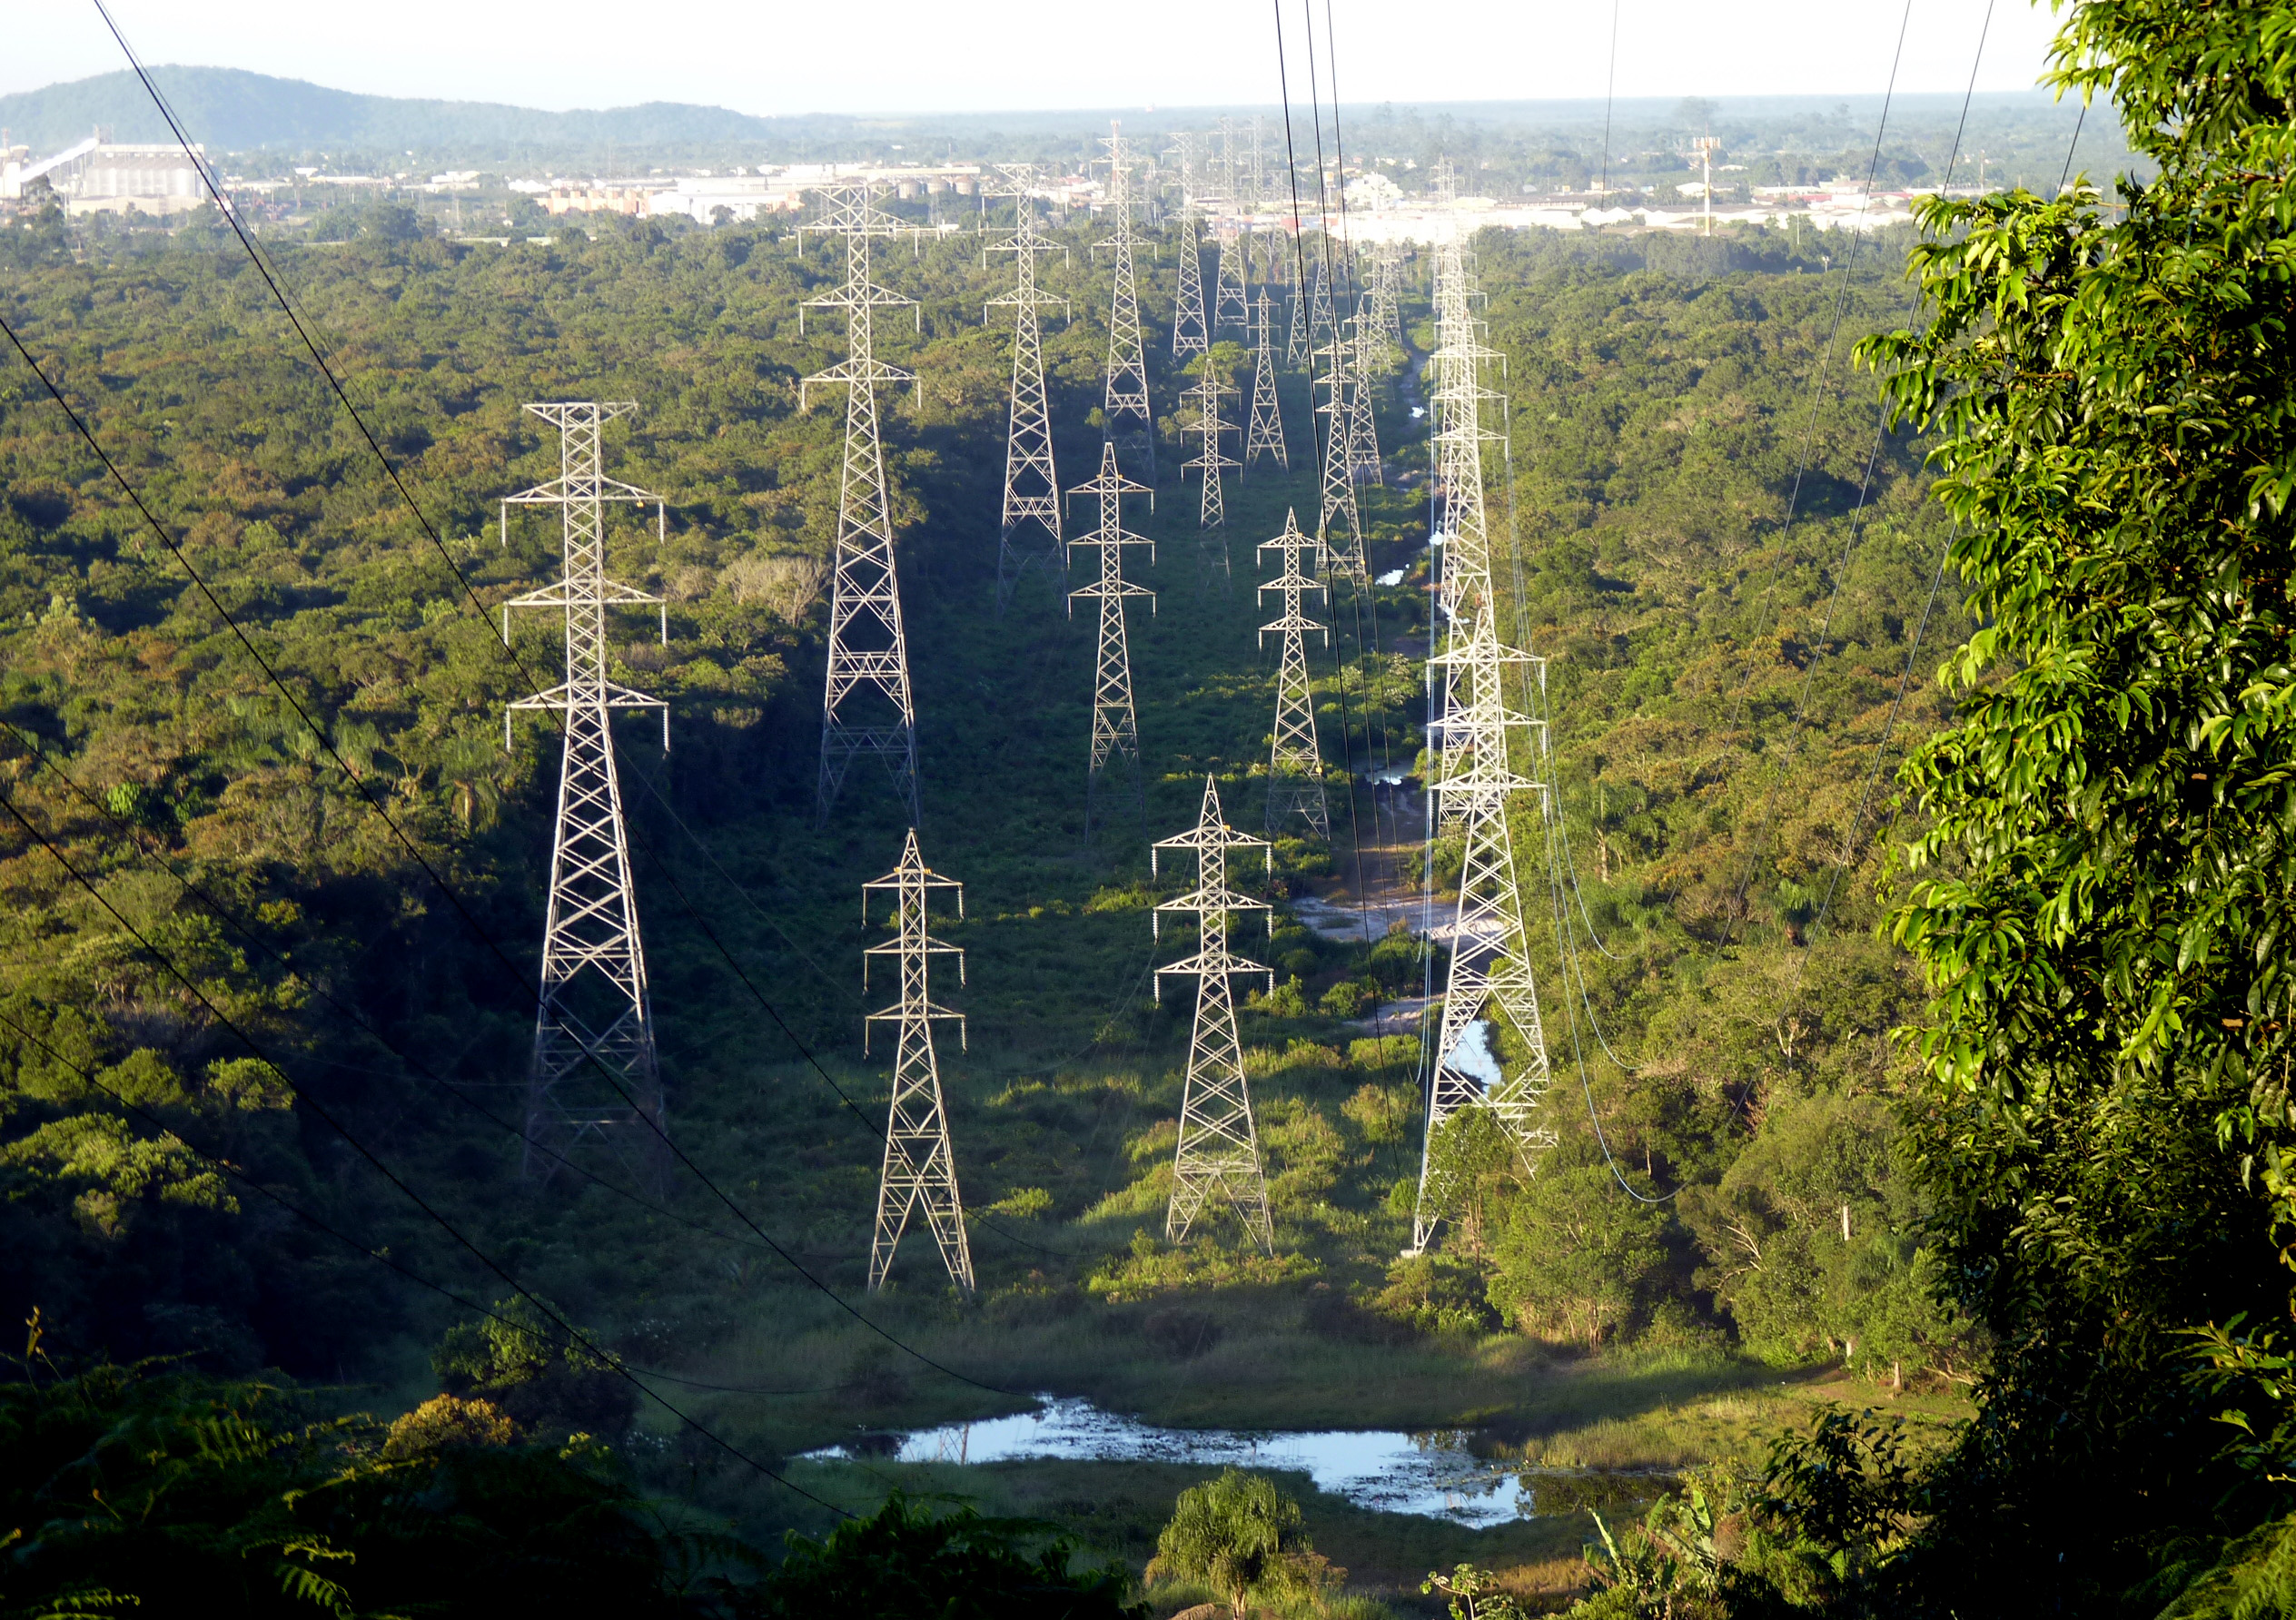
\includegraphics[width=10cm]{./linhaservidao}
	\caption{Faixa de Servidão} \label{linhaservidao}
	\caption*{Fonte: ???}
\end{figure}

\begin{figure}[!ht]
	\centering
	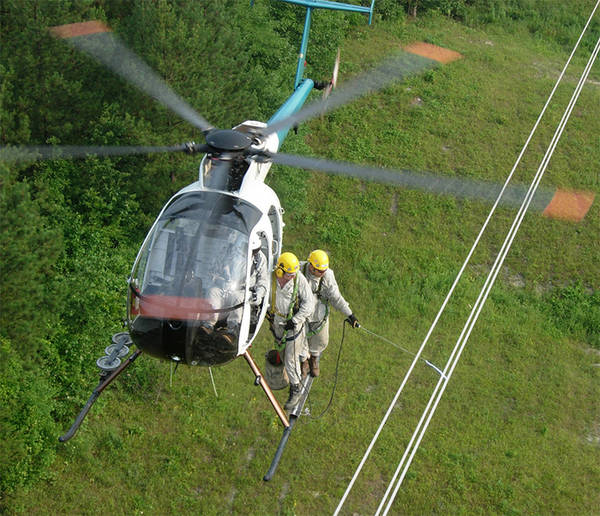
\includegraphics[width=10cm]{./insphelic}
	\caption{Inspeção de uma linha de transmissão} \label{lineinspection}
	\caption*{Fonte: ???}
\end{figure}

Com base no cenário mencionado, foram desenvolvidos diversas propostas de soluções, desde robôs que se movimentam utilizando a LT como cabo guia até UAV's para realizarem as inspeções.

No trabalho de \citeonline{geral}, é abordado o desenvolvimento de um sistema de inspeção visual embarcado em uma aeronave não tripulada, no qual é realizado um vôo de longa distância com uma aeronave pilotada remotamente. O sistema de inspeção conta com uma câmera RGB e uma câmera IR que transmitem as imagens em tempo real para a estação em que o piloto está. A vantagem da utilização de UAV's é que o mesmo pode cobrir longas distâncias, entretanto é necessário manter uma certa distância da LT para que a aeronave possa operar sem riscos de colisão. A desvantagem de se ter esse afastamento é que há uma degradação na qualidade da imagem térmica, dessa forma perdendo detalhes importantes da inspeção. A aeronave pode ser observada na Figura \ref{uav}
\begin{figure}[!ht]
	\centering
	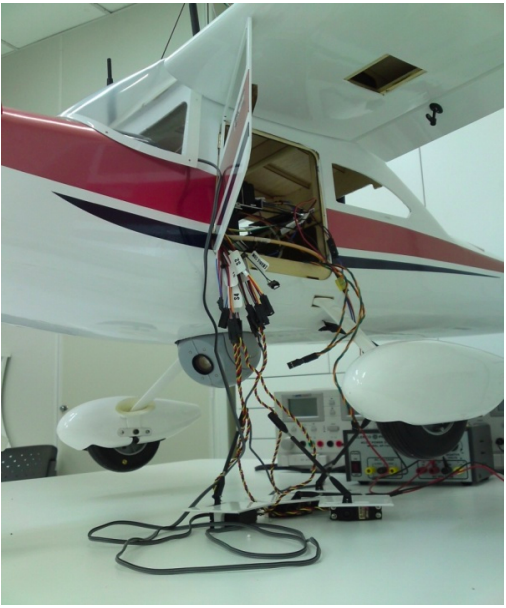
\includegraphics[width=10cm]{./uav}
	\caption{Delta III - UAV para inspeção de LT} \label{uav}
\end{figure}

%não entendi o contexto na abordagem do trabalho ADABO(2014)

De acordo com o que foi abordado, neste trabalho de conclusão de curso, seguindo a metodologia TheoPrax, é proposto o desenvolvimento do sistema de percepção de um robô móvel para inspeção de linhas de transmissão ELIR. O robô se irá se deslocar ao longo do cabo de alta tensão em busca de pontos quentes utilizando uma câmera térmica e verificando se há objetos próximos dos cabos com um sonar. Esses dados serão armazenados com a adição das coordenadas do robô fornecidas por um GPS e horário da detecção. O sistema irá conter outros sensores para compor toda a sua funcionalidade e serão abordados em mais detalhes nesse documento.

%somente no final vc aborda os outros sensores e de forma rápdia


%--------- NEW SECTION ----------------------
\section{Objetivos}
\label{sec:obj}

O  objetivo geral deste  trabalho   é  desenvolver o sistema de percepção para o robô de inspeção de linhas de transmissão ELIR (Electrical Line Inspection Robot).


\subsection{Objetivos Específicos}
Os objetivos específicos do trabalho são:
\label{ssec:objesp}

\begin{itemize}
\item Desenvolver algoritmo para deteção de pontos quentes;
\item Desenvolver o sistema georeferenciamento do robô;
\item Elaborar o sistema de segurança do robô (Análise de temperatura, consumo e Capacidade da Bateria);
\item Construir interface de comunicação com o usuário para apresentar as informações de segurança do robô, informação dos atuadores e todas as ocorrências da missão.
\end{itemize}

%--------- NEW SECTION ----------------------
\section{Justificativa}
\label{sec:justi}

Segundo \citeonline{rangel2009sistema}, a inspeção de linhas de transmissão constantemente é executada através de aeronaves tripuladas. Para \citeonline{lagesoliveira}, este tipo de atividade é considerada de alto risco por conta da baixa altitude das aeronaves e a sua proximidade com as linhas de alta tensão %e se torna ainda mais agravante a depender das condições geográficas e climáticas do local de trabalho.
%melhorar a frase em comentário

A proximidade das aeronaves com as linhas de alta tensão é necessária para realizar a inspeção térmica. Nestas inspeções câmeras infravermelhas são utilizadas para captar a radiação emitida pelas linhas de transmissão, estruturas e elementos. Esta informação é fundamental detecção de pontos quentes na linha e quanto mais quente o ponto, mais susceptível ele está a falha.

A fim de garantir a disponibilidade no fornecimento de energia elétrica, a manutenção de linhas de alta tensão são realizadas de forma preventiva e sistemática, ou seja, a inspeção é realizada com uma certa periodicidade, %tornando-se assim além um de serviço de alto risco também um serviço de alto custo.
%não há subsídios para afirmar isso, onde vc coletou esta informação?

Um dos fatores que mais impactam na manutenabilidade das linhas de transmissão é o desconhecimento do local exato de falha. O tempo gasto para a equipe de manutenção percorrer extensas distâncias na procura do local de falha, torna a manutenção de linhas um atividade de longa duração. Quanto maior o tempo sem abastecimento de energia, maior o transtorno para a população principalmente em regiões com alta demanda, o que pode acarretar em multas para as concessionárias de energia.

A utilização de robôs móveis para inspeção de linhas de alta tensão ganham destaque a partir dos avanços tecnológicos no século XX. Eles são considerados como soluções tecnológicas, uma vez que substituem o trabalho humano em atividades de risco, além disso podem possuir um sistema de sensoriamento capaz de fornecer informações diversas, de acordo com a necessidade do usuário.

O desenvolvimento de robôs para inspeção de LT não só são justificáveis pelo grau de criticidade das linhas mas também por constituírem o resultado de um desenvolvimento tecnológico, gerando pesquisa e desenvolvimento nas instituições e contribuindo para o crescimento científico de todos os envolvidos.



%--------- NEW SECTION ----------------------
\section{Requisitos do cliente}
\label{sec:reqc}

O desenvolvimento do sistema de percepção para o robô ELIR teve como fundamento os requisitos técnicos proposto pelo cliente do projeto. Os requisitos estão apresentados detalhadamente nos tópicos a seguir.
    
    \begin{itemize}
    	\item{\textbf{Inspeção de Temperatura dos cabos, estrutura e obstáculos}}: Devem ser disponibilizadas as informações de medição de temperatura dos cabos, estrutura da linha e de seus obstáculos. Esses dados devem ser obtidos através da câmera térmica para inspeção
    	\item{\textbf{Georreferenciamento dos eventos}}: Todos os eventos de detecção de pontos quentes, sobretemperatura e sobrecorrente devem ser sinalizados em um \textit{logfile} informando a data, horário e coordenadas geográficas obtidos pelo GPS.
    	\item{\textbf{Disponibilizar os videos dos eventos}}: A inspeção realizada pela câmera térmica deve ser disponibilizada em tempo real na interface gráfica do robô.
    	\item{\textbf{Identificação de posicionamento da garra no cabo}}: A fim de garantir a confiabilidade da operação, deve ser realizado uma verificação do alinhamento das garras no cabo da linha de alta tensão.
    	\item{\textbf{Inspeção da linha de servidão}}: Devem ser disponibilizadas informações de objetos até sete metros abaixo do robô
    	\item \textbf{Monitorar temperatura do protótipo}: A temperatura da parte interna do protótipo deve ser monitorada para garantir a segurança dos equipamentos eletrônicos presentes.
	\end{itemize}

%--------- NEW SECTION ----------------------
\section{Organização do \thetypework}
\label{section:organizacao}

Este documento apresenta 5 (cinco) capítulos e está estruturado da seguinte forma:

\begin{itemize}

  \item \textbf{Capítulo \ref{chap:intro} - Introdução}: Contextualiza o âmbito no qual a pesquisa proposta está inserida. Apresenta, portanto, a definição do problema, objetivos e justificativas da pesquisa e como este \thetypeworkthree está estruturado;

  \item \textbf{Capítulo \ref{chap:concep} - Conceito do Sistema}: Descreve como o sistema de Percepção é composto, apresenta a especificação técnica, a arquitetura geral do sistema, a arquitetura de software e os requisitos técnicos;
  
  \item \textbf{Capítulo \ref{chap:mat} - Materiais e Métodos}: Apresenta os materiais utilizados no projeto, explica os suportes mecânicos criados, o diagrama elétrico e o desenho da placa desenvolvida, além das especificações de cada funcionalidade do sistema;%o ponto mais importante deste capítulo é a metodologia.
  
  \item \textbf{Capítulo \ref{chap:result} - Resultados}: Apresenta a descrição dos testes unitários e integrados realizados, assim como os resultados obtidos;
 
  \item \textbf{Capítulo \ref{chap:conc} - Conclusão}: Apresenta as conclusões, contribuições e algumas sugestões de atividades de pesquisa a serem desenvolvidas no futuro.

\end{itemize}

